

\documentclass[12pt]{article}

\usepackage{graphicx}
\usepackage[margin=1in]{geometry}


\title{Simple Latex Report}
\author{
       Mike Hull
}

\date{\today}





\begin{document}
\maketitle

\begin{abstract}
This is the paper's abstract \ldots
\end{abstract}

\section{Introduction}
What is this all about 

\paragraph{Outline}
The remainder of this article is organized as follows.
Section~\ref{previous work} gives account of previous work.
Our new and exciting results are described in Section~\ref{results}.
Finally, Section~\ref{conclusions} gives the conclusions.
Lorem Ipsum is simply dummy text of the printing and typesetting industry. Lorem Ipsum has been the industry's standard dummy text ever since the 1500s, when an unknown printer took a galley of type and scrambled it to make a type specimen book. It has survived not only five centuries, but also the leap into electronic typesetting, remaining essentially unchanged. It was popularised in the 1960s with the release of Letraset sheets containing Lorem Ipsum passages, and more recently with desktop publishing software like Aldus PageMaker including versions of Lorem Ipsum.

\section{Previous work}
\label{previous work}
Blah blah blah blah

Someone found an amazing formula, as in Equation \ref{eqn1}.

\begin{eqnarray}
c^2 = a^2 + b^2
\label{eqn1}
\end{eqnarray}

and someone made up a formula, as in Equation \ref{eqn2}.
\begin{eqnarray}
Y_t = \int^\infty_{n=0} \frac{\gamma e^{-x}}{2 \times n}
\label{eqn2}
\end{eqnarray}

\section{Results}
\label{results}
In this section we describe the results. Check out Figure~\ref{fig1}

\begin{figure}[h!]
\centering
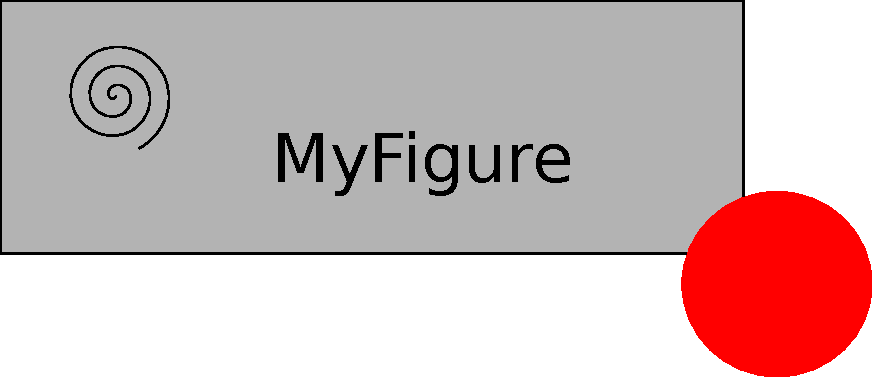
\includegraphics[width=2in]{drawing.pdf}
\caption{A really very interesting figure}
\label{fig1}
\end{figure}

\section{Conclusions}\label{conclusions}
We worked hard, and achieved very little.

\end{document}
